\input{../common}

\begin{document}
  %<*content>
  \lesson{analysis}{23}{Dérivée (TL)}
  
  Le mot << dérivé >> vient du latin << derivare >> qui signifiait << détourner un
cours d'eau >>.\\
Le mot a été introduit par le mathématicien franco-italien Joseph Louis
Lagrange (1736 ; 1813) pour signifier que cette nouvelle fonction dérive
(au sens de "provenir") d'une autre fonction.

La notion de dérivée est une notion fondamentale dans le domaine mathématique de l'analyse numérique. Elle permet d'étudier les variations d'une fonction, de construire des tangentes à une courbe et de résoudre des problèmes d'optimisation.

En sciences, lorsqu'une grandeur est fonction du temps, la dérivée de cette grandeur donne la vitesse instantanée de variation de cette grandeur.

Les dérivées existent un peu partout autour de nous. Même si on ne s'en sert pas dans la vie de tous les jours, la science en a beaucoup besoin. Que ce soit en thermodynamique, en chimie ou en électricité, il existe des tas de formules qui font intervenir des dérivées de fonctions. 


\subsection{Nombre dérivé}


\begin{definition}
 Soit   une fonction  $ f$  définie sur un intervalle I  et $ a $  un réel de I.\\
 On dit que $ f $ est dérivable en $ a $ si  $\displaystyle \lim_{x\to a}{\dfrac{f(x)-f(a)}{x-a} }$   est un réel.\\ Ce réel est appelé \textbf{nombre dérivé} de $ f $  en $ a $ et il est noté\; $ f^{\prime}(a) $.
\end{definition}

\begin{example}

 Soit la fonction $ f $ définie sur $ \Rr $  par \;  $ f(x)=x^{2} $ et  $ a=3 $.\\
 
 On a \; $ \displaystyle\lim_{x\to 3}{\dfrac{f(x)-f(3)}{x-3} }=\displaystyle \lim_{x\to 3}{\dfrac{x^{2}-9}{x-3} }=\lim_{x\to 3}{\dfrac{\paren{x-3}\paren{x+3}}{x-3} }=\lim_{x\to 3}{\paren{x+3}=6 }$ \\
 
 On en déduit que   $ f $ est dérivable en 3 et que le nombre dérivé de $ f $  en 3 est 6 c'est-à-dire \;  $ f^{\prime}(3)=6$.
\end{example}


\subsection*{Interprétation géométrique}
Dans le plan muni  d'un repère orthogonal  $ \oij $,  on note par $\mathscr{C}$   la courbe représentative de la fonction $ f $.\\  Soit A le point de $\mathscr{C}$  d'abscisse $ a. $\\
 La droite T passant par le point  A et de coefficient
directeur $f^{\prime} (a)$  est par définition  \textbf{ la tangente à la courbe} $\mathscr{C}$   au point A.


\begin{center}


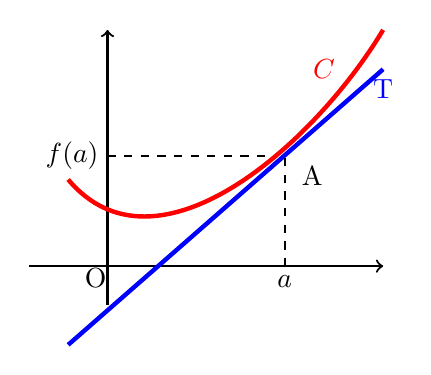
\begin{tikzpicture}[scale= 0.5 ]
\draw (-1,-1)  (7,6);
\draw[->,thick] (-2,0) -- (7,0);
\draw[->,thick] (0,-1) -- (0,6);
\draw[ultra thick, blue]( -1 ,-2)-- (7,5);
\draw[ultra thick,out=-50,in= -121,  red](-1,2.2)to(7,6);
%\draw[ultra thick,out=-120,in=-90,  red](4.1,2.6) to(7,6);
\draw[dashed,thick](4.5,0)--(4.5,2.8);
\node at(5.2,2.3) {A};
\node at(4.5,-0.4) {$a$};
\node at(-0.9,2.8) {$f(a)$};
\draw[dashed,thick](0,2.8)--(4.2,2.8);
\path (5.5,5)  node[ text=red ]{ $\mathscr{C}$ };
\path (7,4.5)  node[ blue ]{ T};
\path (-0.3,-0.3)  node{ O};
\end{tikzpicture}
\end{center}


\textbf{Une équation de la tangente T est:}  \fbox{$y = f^{\prime}(a)(x-a)$}




\begin{example}

Déterminons une équation de la tangente  à la courbe $\mathscr{C}$ de  la fonction $ f $ de  l'exemple précèdent au point d'abscisse 3.

\medskip

 On a $ f(3)=3^{2}=9 $\; et  \; $ f^{\prime}(3)=6$.\\
 Donc en appliquant la formule; on obtient :\; $ y= f^{\prime}(3 )(x-3)+f(3)=6(x-3)+9=6x-9$.\\
 Ainsi la droite affine $ y=6x-9 $ est une équation de la tangente à $\mathscr{C}$   au point d'abscisse 3.
\end{example}



\subsection{Fonction dérivée}


\begin{definition}

\begin{enumerate}
\item[$  \bullet$] 
On dit que $f$  est dérivable sur  l'intervalle I  si elle est dérivable en tout réel de I.

\item[$  \bullet$] La fonction, qui a tout réel $ x $, fait correspondre le nombre dérivé de $f$  en $ x $, quand elle existe,\; s'appelle la
\textbf{fonction dérivée de $f$}  ou encore la   \textbf{dérivée de $f$};  elle est notée $f^{\prime} $.
\end{enumerate}

\end{definition}
 
L'ensemble de définition de $ f^{\prime} $ est appelé  \textbf{ ensemble de dérivabilité de $ f $}.

\subsection{Dérivées des fonctions usuelles}

 \begin{center}
\begin{tabularx}{\textwidth}{|X|X|X|}
\hline
\textbf{Fonction} $f$  &\textbf{ dérivée  } $f^{\prime} $ & \textbf{ Ensemble de dérivabilité} \\ 
\hline
$f(x)= k $,\; \;  $k$  un réel.  & $ f^{\prime}(x)=0 $& $ \Rr $   \\
\hline
$f(x)= x$   & $f^{\prime}(x)=1 $   & $ \Rr $  \\
\hline
$f(x)= x^{n} $,\ \;  $n \in \Zze$    & $ f^{\prime}(x)=n x^{n-1} $ &  $ \Rre, si\;\; n<0 $ \; et\;  $ \Rr, si\,n>0 $   \\
\hline
$f(x)= \dfrac{1}{x} $  & $ f^{\prime}(x)=~-\dfrac{1}{x^{2}} $  &  $\Rre $   \\
\hline
$f(x)= \sqrt{x} $  &  $f^{\prime}(x)= \dfrac{1}{2\sqrt{x}} $ &  $\Rrep$  \\
\hline
$f(x)= ax $    & $ f^{\prime}(x)=a $ &  $\Rr$   \\
\hline
$f(x)=ax+b $    & $f^{\prime}(x)=a $  &  $\Rr$  \\
\hline
\end{tabularx}
\end{center}


\bigskip
\subsection{Formules de dérivations}
Soient $u $ et $v $ deux fonctions dérivables, \; $ n\in\Zze $ \; et\;  $ k\in\Rr $.\\


\begin{tabularx}{\textwidth}{|X|X|X|X|X|X|X|X}
\hline 
\textbf{\color{blue}Fonction }& $ ku $ &$ u+v $ & $ uv $ & $\frac{u}{v}$ & $\frac{1}{v} $ & $ \sqrt{u} $ &  $ u^{n} $ \\     
\hline 
\textbf{\color{blue}Dérivée} & $ ku' $ & $ u'+v' $ & $u'v+ v'u  $ & $ \frac{u'v- v'u }{v^{2}} $ &  $- \frac{v'}{v^{2}} $ & $ \frac{u'}{2\sqrt{u}} $ & $ nu'u^{n-1} $  \\    
\hline
\end{tabularx}
\begin{remark} 
Ces formules  sont à apprendre par coeur. \\
En particulier, la dérivée d'un produit (ou d'un quotient) n'est pas égale au produit (ou au quotient) des dérivées.
\end{remark}


\begin{example}

Calculons la dérivée de chacune des  fonctions suivantes.


\begin{enumerate}
\item $ f(x)=x^{4} +x^{3}-x^{2}-3x+7$
\item $ g(x)=-8x^{3}+2x^{2} +x-12 $
\item $ h(x)=\paren{5x-1}\sqrt{x} $
\item $ k(x)= \frac{3x^{2}-2x+1}{2x-3} $
\end{enumerate}



\end{example}


\begin{proof}
\begin{enumerate}
\item On a:\;  $ f^{\prime}(x)=4x^{3} +3x^{2}-2x-3 +0=4x^{3} +3x^{2}-2x-3$
\item $ g^{\prime}(x)=-8\times 3x^{2}+2\times2x +1-0 =-24x^{2}+4x +1$
\item   Pour $ h(x)=\paren{5x-1}\sqrt{x} $\\
 On pose $ u= 5x-1$ \; et  \;$ v=\sqrt{x} $.\\
Donc $ u^{\prime}=5 $\; et\;  $ v^{\prime}= \frac{1}{2\sqrt{x}}$\\
Ainsi \; $ h^{\prime}(x)=5 \sqrt{x}+ \frac{1}{2\sqrt{x}}\times \paren{5x-1}=\frac{10x+5x-1}{2\sqrt{x}}=\frac{15x-1}{2\sqrt{x}}$
\item  Pour $ k(x)= \frac{3x^{2}-2x+1}{2x-3} $\\
Posons $ u=3x^{2}-2x+1 $\; et \; $ v=2x-3 $\\
Donc  $ u^{\prime}=6x-2 $\; et \; $ v^{\prime}=2 $\\

Ainsi \; $ k^{\prime}(x)= \frac{\paren{6x-2}\paren{2x-3}-2\paren{3x^{2}-2x+1}}{\paren{2x-3}^{2}}=\frac{6x^{2}-18x+4}{\paren{2x-3}^{2}}$
\end{enumerate}

\end{proof}

\begin{remark}

 L'ensemble de dérivabilité d'une fonction polynôme ou d'une fonction rationnelle  est égal à l'ensemble de définition.
\end{remark}

\subsection{Dérivée d'une fonction composée}



\begin{theorem}

Soient   $f $ et $ g$ deux fonctions dérivables.
   \[ \text{On a:}\quad (gof)^{\prime}(x)=f^{\prime}(x)\times g^{\prime}\croch{f(x)}\]
\end{theorem}



\begin{corollary}
\begin{enumerate}
\item  Pour $ a>0 $\\
 La fonction \; $ x\longmapsto \sqrt{ax+b} $ \; est  définie sur  $ \intfo{-\dfrac{b}{a}}{\pinf} $ ,  dérivable sur $ \intoo{-\dfrac{b}{a}}{\pinf} $ et a pour dérivée:
 
 \[  \paren{\sqrt{ax+b}}^{\prime}(x)=\dfrac{a}{2\sqrt{ax+b}} \]
 
\item  Pour $ a<0 $\\
 La fonction \; $ x\longmapsto \sqrt{ax+b} $ \; est  définie sur  $ \intof{\minf}{-\dfrac{b}{a}} $ ,  dérivable sur $ \intoo{\minf}{-\dfrac{b}{a}} $ et a pour dérivée:
 
 \[ \paren{\sqrt{ax+b}}^{\prime}(x)=\dfrac{a}{2\sqrt{ax+b}} \]


\begin{example}
\begin{itemize}
\item[$  \bullet$] $ f(x)=\sqrt{2x-5} $ est dérivable sur   $ \intoo{\dfrac{5}{2}}{\pinf} $ et pour tout $ x> \frac{5}{2} $,\;                                                                $  f^{\prime}(x)= \dfrac{2}{2\sqrt{2x-5}}=~\dfrac{1}{\sqrt{2x-5}}$\\
\item[$  \bullet$]$ g(x)=\sqrt{-x+1} $ est dérivable sur   $ \intoo{\minf}{1} $ et pour tout $ x< 1 $,\;  $  g^{\prime}(x)= \dfrac{-1}{2\sqrt{-x+1}}$
\end{itemize}
\end{example}

\item Cas général: si u est une fonction dérivable et strictement positive alors on a :\; $ \paren{\sqrt{u}}^{\prime}=\frac{u^{\prime}}{2\sqrt{u}} $.
\begin{example}
\begin{itemize}
\item  Si $ f(x)=\sqrt{2x^{2}-x+1}\; $  alors  $ \; f^{\prime}(x)= \frac{4x-1}{2\sqrt{2x^{2}-x+1}}$\\
\item  si $ g(x)=\sqrt{x^{2}+7} $ \; alors \;  $ g^{\prime}(x)= \dfrac{2x}{2\sqrt{x^{2}+7}}= \dfrac{x}{\sqrt{x^{2}+7}}$
\end{itemize}

\end{example}

\textbf{Formule}
\[  \paren{\sqrt{ax^{2}+bx+c}}^{\prime}=\dfrac{2ax+b}{2\sqrt{ax^{2}+bx+c}}\]


\bigskip

\item La fonction  $ u^{n} $ a pour dérivée  $ nu'u^{n-1} $.

\begin{example}
\begin{itemize}
\item[$  \bullet$]  si $ f(x)=\paren{5x+1}^{3} $ \; alors \;  $ f^{\prime}(x)= 3\times 5\paren{5x+1}^{2}=15\paren{5x+1}^{2}$.


\item[$  \bullet$]  Si $ g(x)=\paren{\sqrt{x}+3}^{2} $ \; alors \; $  g^{\prime}(x)= 2\times \dfrac{1}{2\sqrt{x}}\paren{\sqrt{x}+3}=\dfrac{\sqrt{x}+3}{\sqrt{x}}$


\end{itemize}

\end{example}
\end{enumerate}
\end{corollary}

\subsection{Utilisation de la dérivée}

\subsection*{Dérivée et sens de variation}
\begin{theorem}
Soit $ f $ une fonction dérivable sur un intervalle $ I. $
\begin{itemize}
\item Si $ f $ est positive sur I alors  $f$ est  croissante sur $I$ 
\item Si $ f $ est négative sur I alors  $f$ est  décroissante sur $I$ 
\item Si  $ f $ est nulle  sur I alors  $f$ est  constante sur $I$. 
\end{itemize}
\end{theorem}
\begin{example}
Considérons la fonction $ f $ définie par $ f(x)=x^{3}-3x$.\\
$ f $  est continue et dérivable sur $ \Rr $  et  $ f^{\prime}(x)=3x^{2}-3$.\\
La dérivée est du second degré , cherchons ses racines.\\ Posons $3x^{2}-3=0   $ donc $ 3x^{2}=3 $ c'est-à-dire $ x^{2}=1$ d'où $x=-1 $ ou $x=1 $.\\
 On en déduit que $ f^{\prime} $ est positive sur les intervalles $ \intof{\minf}{-1} $  et $ \intfo{1}{\pinf} $  d'où $ f $ est croissante sur ces mêmes intervalles.\\
$ f^{\prime} $  est négative sur $ \intff{-1}{1} $ d'où $ f $ est croissante sur $ \intff{-1}{1} $. \\On a le tableau de variation de $ f $ suivant:
\begin{center}
$\begin{array}{c|cccc}
x & -\infty & -1 & 1 & +\infty \\
\hline
f'(x) &      & + & 0 & - \\
f(x)  & \nearrow & 2 & \searrow & -2 \nearrow
\end{array}$

\end{center}
$-2$   et  $2 $ sont respectivement maximum et minimum de la fonction $ f $: ce sont des extremums.\\
\textbf{Rappel}\\ Si en un réel $ a $, la dérivée s'annule en changeant de
signe, alors le réel $ f(a) $ un extremum de $ f $.
\end{example}
\begin{example} 
Soit la fonction $ g $ définie par $ g(x)=\dfrac{x^{2}+x-1}{x-1} $ pour $ x\neq1 $.\\
On a:\; $ g^{\prime}(x)=\dfrac{x^{2}-2x}{\paren{x-1}^{2}} =\dfrac{x(x-2)}{\paren{x-1}^{2}}$.\\ Le signe de $ g^{\prime}(x) $ dépend de celui de $ x(x-2) $  car $ \paren{x-1}^{2}>0 $.\\ Or $ x(x-2) $ est du second degré et $ x(x-2)=0 $  si $ x=0$ ou $x=2 $.\\ Donc $ x(x-2) \geq0$  si $ x\in\intof{\minf}{0} \cup \intfo{2}{\pinf}$\; et $ x(x-2)\leq 0$  si             $ x\in\intff{0}{2} $.\\
On a le tableau de variation de $ g $ suivant:
\end{example}
\begin{center}
\begin{tikzpicture}[scale=0.8]
\tkzTabInit[]
{$x$ /1, $g'(x)$ /1,$g(x)$ /2}
{$-\infty$ , $ 0 $, $1$ , $2$ , $+\infty$}
\tkzTabLine{,+,z,-,d,-,z,+,}
\tkzTabVar{-/$-\infty$,+/$1$,-D+/$-\infty$ / $+\infty$ ,-/$5$, +/$+\infty$}
%\tkzTabVal{1}{2}{0.4}{}{}
\end{tikzpicture}

On a $ g'0)=1  $\; et \; $ g(2)=5 $
\end{center}
 Le nombre 1 est un maximum local de $ g $ tandis que le nombre réel 5 est un minimum local de $ g $.
\subsection*{Notion de bijection}
\begin{theorem}
 Si f est définie continue, strictement croissante ( ou strictement décroissante)
sur  un intervalle I alors f réalise une bijection de I sur f(I).

\end{theorem}

\begin{example}

D'après le tableau de variation de l'exemple précèdent,\\
$ \bullet $ $ f $ est une bijection de $ \intof{\minf}{-1} $ sur $ \intof{\minf}{2} $\\
$ \bullet $ $ f $ est une bijection de $ \intff{-1}{1} $ sur $ \intof{-2}{2} $\\
$ \bullet $ $ f $ est une bijection de $ \intfo{1}{\pinf} $ sur $ \intfo{2}{\pinf} $

\end{example}

 
  %</content>
\end{document}
